\section{MOTIVATION OF CUBIC SPLINE INTERPOLATION}

Given $n+1$ data points $(x_1, y_1), (x_1, y_1), ..., (x_{n+1}, y_{n+1})$, we seek to construct a smooth curve that passes through all data points. The easiest method is linear interpolation, however linear interpolation does not produce a smooth curve. Another method is to use a polynomial of high degreewhich tends to produce unwanted oscillations.

Cubic spline interpolation is a method that sits in between, provides smooth curve of second order and does not oscillate too much (limited to third order polynomials)

\section{DEFINITION OF CUBIC SPLINE INTERPOLATION}

Given $n+1$ data points $(x_1, y_1), (x_1, y_1), ..., (x_{n+1}, y_{n+1})$, for every $i = 1, ..., n$, we choose a polynomial (spline)
$$
	f_i(x) = a_i (x - x_i)^3 + b_i (x - x_i)^2 + c_i (x - x_i) + d_i
$$

for each interval $[x_{i-1}, x_i]$, so that it satisfies the following constraints
\begin{enumerate}
	\item (goes through all points) $f_i(x_i) = y_i$ and $f_i(x_{i+1}) = y_{i+1}$, that is
	\begin{align*}
		y_i  &= d_i\\
		y_{i+1} &= (x_{i+1} - x_i)^3 a_i + (x_{i+1} - x_i)^2 b_i + (x_{i+1} - x_i) c_i + d_i
	\end{align*}
	for every $i = 1, ..., n$
	
	\item (continuity of first derivative) $f_i'(x_{i+1}) = f_{i+1}'(x_{i+1})$, that is
	$$
		3 (x_{i+1} - x_i)^2 a_i + 2 (x_{i+1} - x_i) b_i + c_i = c_{i+1} 
	$$
	for every $i = 1, ..., n$
	
	\item (continuity of second derivative) $f_i''(x_{i+1}) = f_{i+1}''(x_{i+1})$, that is
	$$
		6 (x_{i+1} - x_i) a_i + 2 b_i = 2 b_{i+1}
	$$
	for every $i = 1, ..., n$
\end{enumerate}

In total, we have $4n-2$ constraints and $4n$ variables. The other two constraints (boundary conditions) will be introduced in the next section 

\section{TWO METHODS FOR CONSTRUCTING CUBIC SPLINE INTERPOLATION}

\subsection{NATURAL SPLINE}

Natural spline is used when there is no information about \textit{derivative} of the curve at $x_1$ and $x_{n+1}$, that is to set
$$
	f_1''(x_1) = 0 \text{ and } f_n''(x_{n+1}) = 0
$$

That induces two constraints

$$
	2 b_1 = 0 \text{ and } 6(x_{n+1} - x_n) a_n + 2 b_n = 0
$$

\subsection{CLAMPED SPLINE}

Clamped spline is used when there is information about the \textit{first derivative} of the curve at $x_1$ and $x_{n+1}$
that is to set
$$
	f_1'(x_1) = f'(x_1) \text{ and } f_n'(x_{n+1}) = f'(x_{n+1})
$$

That induces two constraints

$$
	c_1 = f_1'(x_1) \text{ and } 3 (x_{n+1} - x_n)^2 a_n + 2 (x_{n+1} - x_n) b_n + c_n =  f'(x_{n+1})
$$


\section{MATLAB CODE AND NUMERICAL EXAMPLES}

\subsection{NUMERICAL EXAMPLES}

Consider the following data points
$$
	(0, 7), (1, 1), (2, 2), (3, 2)
$$

with boundary conditions $f'(x_1) = f'(0) = 5$ and $f'(x_{n+1}) = f'(3) = -5$. The figure below describes the two curves constructed from natural cubic spline (not using boundary condition) and clamped spline.

\begin{figure}[H]
	\begin{center}
		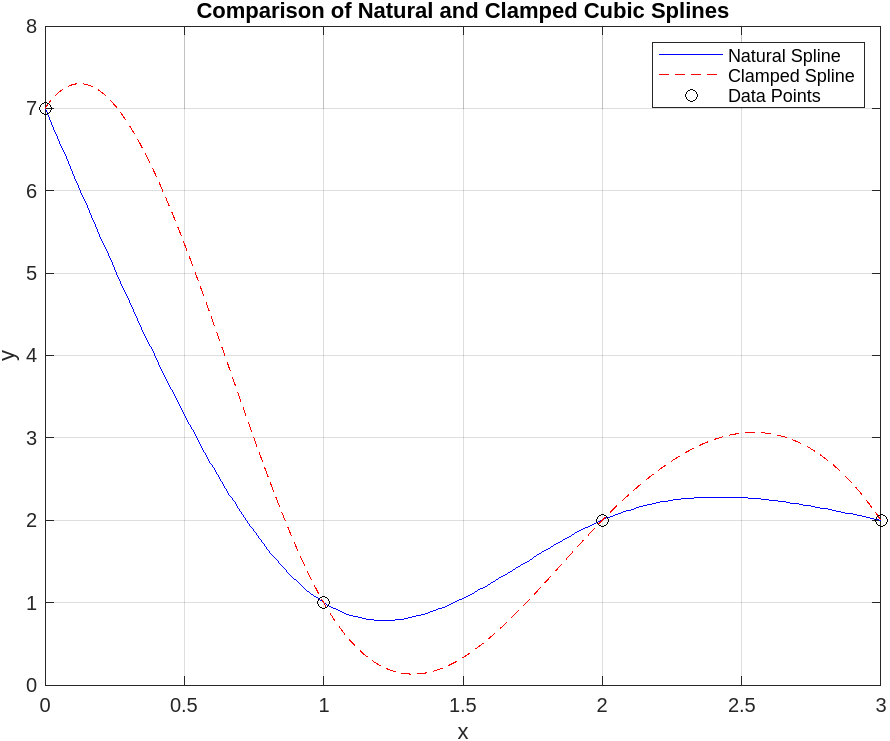
\includegraphics[width=8cm]{ma5271.png}
	\end{center}
\end{figure}


\subsection{MATLAB CODE}

\lstinputlisting[language=matlab]{ma5271.m}


